\documentclass{article}
\usepackage{fullpage}
\usepackage{graphicx}
\author{Fergus W. Leahy - 0908622L}

\title{Wireless Sensor Networks Assessed Coursework 2}

\begin{document}
\maketitle{}

\section{Introduction}
The purpose of this report is to discuss the design and implementation of the Twitter-like framework, Tinyblog, for the wireless sensor devices, as well as demonstrate the extent to which the requirements have been fulfilled.  

\section{Design}
The design of the TinyBlog framework is tightly bound by the modularity of TinyOS, where possible the implementation has been split into modules (such as Packet buffers).

Figure \ref{fig:modules} shows the basic wiring of different modules in the system. A full diagram of the wiring can be found in the appendicies.
\begin{figure}[htb!]
\centering
\includegraphics[scale=0.4]{TinyBlog_wiring.jpg}
\caption{TinyBlog wiring}
\label{fig:modules}
\end{figure}  

The system modules include: 
\begin{itemize}
	\item Active messaging - used to communicate over the radio
	\item Light/Temp sensors - used to create mood data
	\item Timers - used for various tasks which must be triggered repeatedly, such as retrieving sensor readings for the mood
	\item LEDS - used to signify activity on the network, i.e., blink red for tweet forwarded
\end{itemize}

The TinyBlog modules include:
\begin{itemize}
	\item Follow List(Circular Queue) - used to store the users which the node is following
	\item Packet Buffer - used to store the metadata (src, seqno) of recent packets received (to stop broadcast storm)
	\item Tweet Queue - used to store the messages of tweets received or ready to transmit on the network(depending of scenario).
	\item Interest Table - used to create a cache of any recently seen interests for tweets(used for scenario 2).
\end{itemize}


\section{Requirements fulfilled}
\subsection{Transferred data format}
\begin{itemize}
	\item Use of specified data format - TinyBlogMsg.h has been included and used where necessary
	\item Message body of 100 bytes - DATA\_SIZE has been modified to 100 bytes and TOSH\_DATA\_LENGTH is set through a compile time flag to accommodate the extra bytes
	\item End of message - The host application automatically truncates a message which is too long and sets nchars to the correct number of chars.
\end{itemize}

\subsection{Host-side Application}
The host-side application is a command line application written in Java, this was chosen due to the familiarity of the author with Java, as well the documentational support and examples of how the application should be created.

\begin{itemize}
	\item Client communicates to the mote application via the base station
	\begin{itemize}
		\item the application allows users set the destination of their actions to their specific node, this is done by calling, \textit{connect} \textless nodeid\textgreater
	\end{itemize}
 	\item Allow users to post tweets
 	\begin{itemize}
 		\item the application allows users to post tweets to the node which it is connected to.
 	\end{itemize}
 	\item Allow users to follow tweets from other users
 	\begin{itemize}
 		\item The host-side application allows a user to indicate which nodes to follow for tweets, using the command: \textit{follow} \textless nodeid\textgreater, where nodeid is the node the user wants to follow. This is then sent as a message to the mote application which then updates its follow list. After which it will then save any messages which it receives if the mote ids are in the list.
 	\end{itemize}
 	\item Poll the state of the buffer
 	\begin{itemize}
 		\item The host-side application can request all the tweets the node has received, these are displayed on the host-side application.
 	\end{itemize}
 	\item Receive a message from someone followed and display on client
 	\begin{itemize}
 		\item When a new message has arrived on the node, after it is processed it is then saved and transmitted the the base station where the host-side application receives and displays the tweet. 
 	\end{itemize}
 \end{itemize} 


\subsection{Mote application}
\begin{itemize}
	\item Multi-hop, packet forwarding
	\begin{itemize}
		\item The mote application fully supports robust packet forwarding and avoids contributing to broadcast storms. This is done through the correct use of using the TTL field in the data structure, as well as using a buffer of previously seen packet meta data. This buffer is used so that when new packets arrive they can be checked and if a match is found in the buffer they are dropped immediately, as they must have been re-broadcasted. The buffer is a circular data structure storing 32 packets metadata, so when full it overwrites the oldest packet. This makes a compromise between the size of the buffer and the amount of ``recent'' packets which can be recognised.
	\end{itemize}
	\item Support Minimal Protocol commands
	\begin{itemize}
		\item All minimal commands have been implemented and depending on the scenario the functionality changes.
		\begin{itemize}
			\item Post tweet
			\begin{itemize}
			 	\item In scenario 1, when a post tweet is received from the base station, the mood and source mote id is set, and then the tweet is broadcast across the network. If a mote receives a new, unseen post tweet from a mote which is mote which is not the base station then it checks if it is follow the user which created it, if so it saves it locally and then transmits it to the base station. Regardless of whether the tweet was followed, it is broadcasted back on to the network if it has not expired its TTL.
			 	\item In scenario 2, when a post tweet is received from the base station it is just stored locally on the mote, waiting for a get tweet message from another mote. If it receives a post tweet message from another mote on the network it checks to see if it can route it, (further discussed in the \ref{sec:dd}), if so then it sends it to the next hop.
			\end{itemize} 
			\item Add user to follow list
			\begin{itemize}
			 	\item In both scenarios, when the host side applications sends a follow user message to the mote, the mote stores the id in its follow list. This follow list is then consulted when either receiving tweets or looking for tweets. 
			 \end{itemize} 
			 \item Retrieve new tweets
			 \begin{itemize}
			 	\item 
			 \end{itemize}
		\end{itemize}

	\end{itemize}
\end{itemize}

\section{Testing \& Evaluation}


\section{Appendices}
\begin{figure}[htb!]
\centering
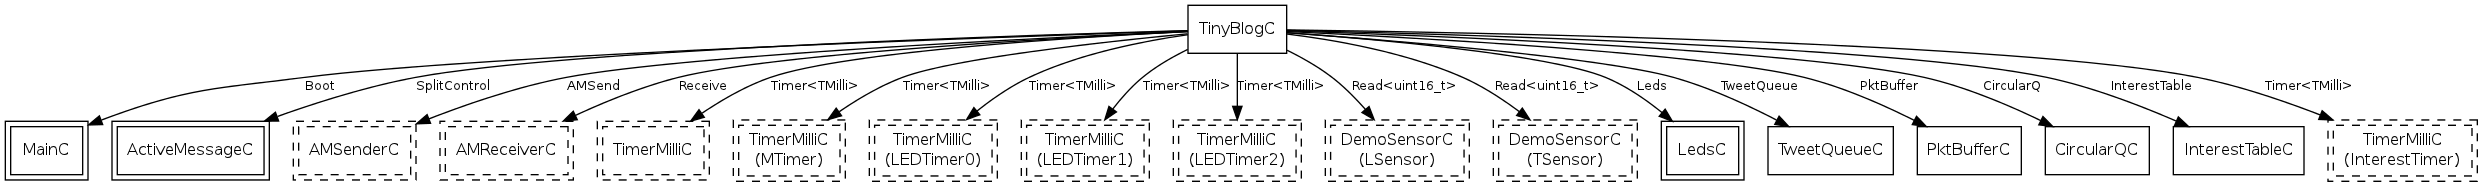
\includegraphics[scale=.27,angle=90]{TinyBlogAppC.png}
\label{fig:fullWiring}
\caption{TinyBlog wiring, created using nesdoc}
\end{figure}



\end{document}